\section{Results}
Test which sample with which algorithm?

\subsection{Matconvnet}
\subsubsection{Bragg peaks}
\subsubsection{Molecule projections}
A traditional Convolutional Neural Network (CNN) is parameterized by floating point weights and biases
and takes floating point data as input. In many cases, the floating point representation of these
parameters and input is more than necessary. The use of a more compact representation of the
parameters and input allows CNNs to be deployed on energy efficient architectures that operate with a
few bits and much lower memory footprint. This work focuses on data reduction and quantization schemes
that can be applied to a trained CNN for classifying scienti c simulation data. We show that each
neuron and synapse can be encoded with only one byte to maintain accuracy above 98\%.
\begin{figure}[h]
\centering
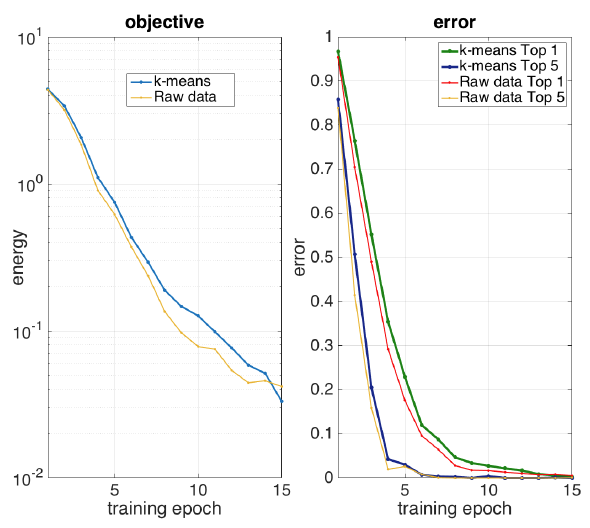
\includegraphics[width=\linewidth]{img/joao3.png}
\caption{Simulation results for the network.}
\label{fig_sim}
\end{figure}


64 by 64 projection images of TFIID along 9 viewing angles with random perturbation, noise free);

\begin{table}[]
\centering
\caption{My caption}
\label{my-label}
\begin{tabular}{|c|c|c|}
\hline
 $\Psi\downarrow_i$    & $\Theta\downarrow_i$       & $\phi\downarrow_i$
 \\
 \hline
0.00 & 0.0000 & 0.0000 \\
0.00 & 45.000 & 0.0000 \\
0.00 & 45.000 & 89.975 \\
0.00 & 45.000 & 179.95 \\
0.00 & 45.000 & 269.92 \\
0.00 & 90.000 & 0.0000 \\
0.00 & 90.000 & 59.983 \\
0.00 & 90.000 & 119.97 \\
0.00 & 90.000 & 178.95 \\
\hline
\end{tabular}
\end{table}

\textbf{Classifying 9 views:}
Training images generated from a 3D density map of a transcription factor-II

\textbf{Testing}
100 projection images generated from Euler angles
 chosen randomly from 1 to 9
,  generated randomly (uniform distribution) with
Result: 100\% success rate

\subsubsection{Scattering patterns}
We address the problem of classifying GISAXS patterns from 7 different crystal lattices (classes). We generated 1,000 images with dimensions of 100X100 pixels for each class by varying the lattice parameters as input to a 4 layer CNN to train a classifier. The architecture of this network is adapted from the MNIST classifier used by MatConvNet. We tested the performance of the classifier on
multiple data sets, including samples corrupted with realistic noise levels. We obtained an accuracy that ranged from 82.6\% to 92.29\% depending on the parameters of each test case which we believe is an encouraging result for further extending the use of CNNs for GISAXS as well as other synchrotron based scientific experiments.

\begin{table}[]
\centering
\caption{My caption}
\label{my-label}
\begin{tabular}{|c||c|c|c|}
\hline
Method & dataset1 & dataset2 & noisyDataset \\
\hline
CNN    & 92.29    & 82.60    & 91.57        \\
HOG    & 92.00    & 79.88    & 79.57        \\
\hline
\end{tabular}
\end{table}

\subsection{Neuromorphic computing}
Corelet Laboratory: Corelet Language + Corelet Library (used to configure the neural network)
COMPASS simulator
Available for IBM Blue Gene Q;
Average neuron spiking rate 8.1 Hz (388 times slower than real time);
Support both MPI and OpenMP and PGAS;

The job of a TrueNorth programmer is to translate a desired computation into a specified network of neurosynaptic cores, its inputs and outputs through corelets
In this project, we will produce corelets for several image analysis and pattern recognition problems relevant to DOE science applications

Challenges: Can we build a computer that works like a brain?
Quick classification, pattern recognition
Low power
Fault tolerant
Easy to program


%\begin{figure}[h]
%\centering
%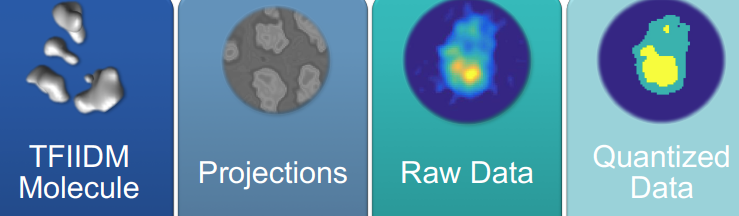
\includegraphics[width=\linewidth]{img/joao1.png}
%\caption{Simulation results for the network.}
%\label{fig_sim}
%\end{figure}

\begin{figure}[h]
\centering
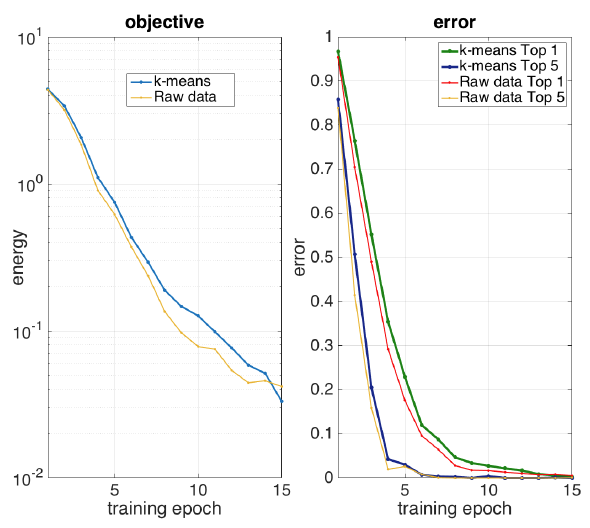
\includegraphics[width=\linewidth]{img/joao3.png}
\caption{Coisas do jao.}
\label{fig:cryem}
\end{figure}

IBM TN settings:
Corelet Programming Environment CPE Version 2.2.160518
CPE + tn-signal-processor to make a model
and run a model on the TrueNorth hardware
Matlab with MatConvNet

Fibers=216,650 samples
Non-fibers=105,120 samples
Each sample = 162 uint8 input (raw = no processing)
How: leverage curated data analyzed using sophisticated computer vision algorithms + user intervention

Preliminary results using the neuromorphic chip IBM TrueNorth
Specs and accuracy:
~3,200 cores < 1 chip = 4096 cores
Model =
Train=70\%; test=30\%
Accuracy = 99.788623\%

What is next:
Interpret Eedn output results
Deploy TN on a testbed at NERSC
Port models to the chip at LBL
Evaluate on new samples coming from ALS

\subsection{NVIDIA DevBox}

pyCBIR is python package that offers a prototype system for user exploration of general image composition. The system enables image-based query to digital imagery archives, returning the top-n pictures that most resembles the query.


%Our search engine builds upon computer vision advances made over the past decade in low-level feature matching, large data handling and object recognition. We demonstrate hierarchical clustering among images semi-cooperatively shot around MIT, automatic linking of flickr photos and aerial frames from the Grand Canyon, and video segment identification for a TV broadcast. Moreover, our software tools incorporate visible vs infrared band selection, color content quantization and human face detection. Ongoing and future extensions of this image search system are discussed.


\begin{figure*}[!t]
\centering
\subfloat[Case I]{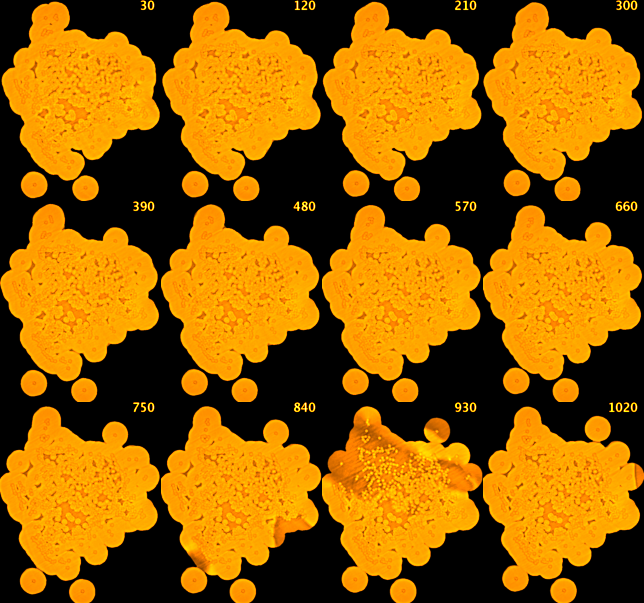
\includegraphics[width=.439\linewidth]{img/fiberMontage.png}
\label{fig_first_case}}
\hfil
\subfloat[Case II]{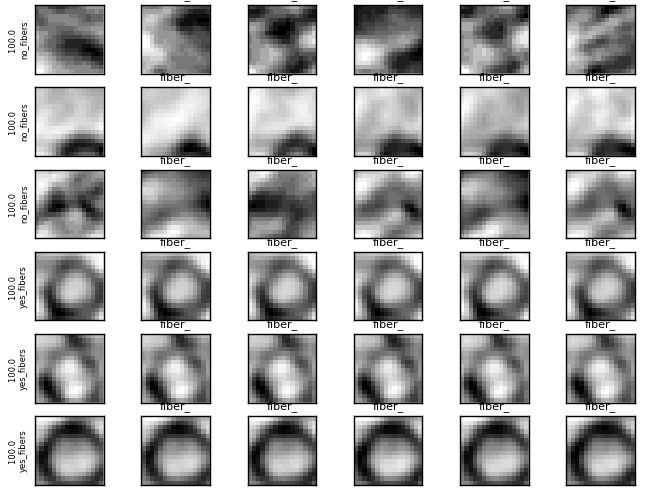
\includegraphics[width=.54\linewidth]{img/fiberCBIR.png}
\label{fig_second_case}}
\caption{Using TensorFlow: Dataset with more than three hundred thousand samples, used to train a deep
learning algorithm in order to separate fiber profiles (left) from other regions (right) as they
appear in micro tomography image from ceramic matrix composites. Accuracy results for this CNN are
99.788623\%, considering stratified training and tests sets, with 70\% and 30\% of the samples
respectively.}
\label{fig:pycbir}
\end{figure*}



% \begin{table}[!h]
% \caption{This is only a place holder for table.}\label{tab:accTari} \centering
% \begin{tabular}{|c||c|c|c|}
%   \hline
%   \multirow{2}{*}{\textbf{Method}} & \textbf{Tari 56} & \textbf{Tari 180} & \textbf{Tari 1000} \\
%    & \textbf{Database} & \textbf{Database} & \textbf{Database} \\
%   \hline
%   Proposed & \textbf{99.84\%} & \textbf{96.66\%} & \textbf{81.60\%} \\
%   \hline
%   ProposedNoConc & 93.82\% & 90.84\% & 73.96\% \\
%   \hline
%   PedrosaA \cite{Pedrosa:2011a} & 43.25\% & 26.40\% & 15.49\% \\
%   \hline
%   PedrosaB \cite{Pedrosa:2011b} & 75.06\% & 61.46\% & 53.35\% \\
%   \hline
%   PedrosaBConc & \textbf{76.48\%} & \textbf{66.13\%} & \textbf{57.83\%} \\
%   \hline
%   TAR & 86.30\% & 84.86\% & 64.27\% \\
%   \hline
% \end{tabular}
% \end{table}
